\documentclass[aspectratio=169]{beamer}
\usepackage[T1]{fontenc}
\usepackage[utf8]{inputenc}
\usepackage{lmodern}
\usepackage{microtype}
\usepackage{xcolor}
\usepackage{tikz}
\usetikzlibrary{positioning, arrows.meta, calc}
\usepackage{fontawesome5}
\definecolor{wurgreen}{HTML}{34B233}
\definecolor{darkgreen}{HTML}{1F6B1E}
\definecolor{darknavy}{HTML}{1A1A2E}
\definecolor{midgray}{HTML}{6B7280}
\definecolor{lightgray}{HTML}{F3F4F6}
\definecolor{lightgreen}{HTML}{E8F7E8}
\definecolor{bodytext}{HTML}{1F2937}
\definecolor{warnred}{HTML}{FEE2E2}
\definecolor{warnborder}{HTML}{EF4444}
\definecolor{codebg}{HTML}{1E1E2E}
\definecolor{codegreen}{HTML}{9ECE6A}
\definecolor{codeblue}{HTML}{7AA2F7}
\definecolor{codeorange}{HTML}{FF9E64}
\definecolor{codegray}{HTML}{C0CAF5}
\usetheme{default}\usecolortheme{default}\usefonttheme{professionalfonts}
\setbeamertemplate{navigation symbols}{}
\setbeamertemplate{itemize items}{\textcolor{wurgreen}{\textbullet}}
\setbeamertemplate{itemize subitem}{\textcolor{midgray}{--}}
\setbeamercolor{frametitle}{fg=white, bg=darknavy}
\setbeamerfont{frametitle}{size=\large, series=\bfseries}
\setbeamertemplate{frametitle}{%
  \begin{beamercolorbox}[wd=\paperwidth, ht=1.1cm, dp=0.2cm, leftskip=0.6cm]{frametitle}
    \usebeamerfont{frametitle}\insertframetitle\end{beamercolorbox}}
\setbeamercolor{background canvas}{bg=white}
\setbeamercolor{normal text}{fg=bodytext}
\setbeamertemplate{footline}{%
  \begin{beamercolorbox}[wd=\paperwidth, ht=0.4cm, dp=0.15cm]{footline}
    \hspace{0.5cm}\textcolor{midgray}{\tiny Introduction to Python · Module 2: Data Structures}%
    \hfill\textcolor{midgray}{\tiny \insertframenumber}\hspace{0.4cm}\end{beamercolorbox}}
\newcommand{\codebox}[1]{\begin{center}
  \begin{tikzpicture}\node[fill=codebg, rounded corners=4pt, inner sep=9pt, text width=0.85\textwidth, text=codegray]{\ttfamily\small #1};\end{tikzpicture}\end{center}}
\begin{document}
{\setbeamertemplate{footline}{}
\begin{frame}[plain]
  \begin{tikzpicture}[remember picture, overlay]
    \fill[darknavy] (current page.south west) rectangle (current page.north east);
    \fill[wurgreen] (current page.south west) rectangle ([xshift=0.45cm]current page.north west);
    \node[anchor=west, text=white, font=\huge\bfseries, text width=13cm] at ([xshift=1.1cm, yshift=1.4cm]current page.west){Introduction to Python};
    \node[anchor=west, text=wurgreen, font=\large, text width=12cm] at ([xshift=1.1cm, yshift=0.2cm]current page.west){Module 2 --- Data Structures};
    \node[anchor=west, text=midgray, font=\small, text width=12cm] at ([xshift=1.1cm, yshift=-1.3cm]current page.west){Lists, dictionaries, tuples, and sets};
  \end{tikzpicture}
\end{frame}}

\begin{frame}{Why We Need Data Structures}
\vspace{0.2cm}
{\small So far each variable held \emph{one} value. But real data comes in \textbf{collections}
--- a list of documents, a table of counts, a set of unique words. Python has built-in
structures for exactly this.}
\medskip
\begin{center}
\renewcommand{\arraystretch}{1.4}
{\small
\begin{tabular}{p{2.3cm}|p{4cm}|p{4.5cm}}
\textbf{Structure} & \textbf{Holds} & \textbf{Example} \\
\hline
\texttt{list} & ordered, changeable & \texttt{["a", "b", "c"]} \\
\texttt{dict} & key $\rightarrow$ value pairs & \texttt{\{"count": 5\}} \\
\texttt{tuple} & ordered, \emph{unchangeable} & \texttt{(52.1, 5.6)} \\
\texttt{set} & unordered, \emph{unique} & \texttt{\{"a", "b"\}} \\
\end{tabular}}
\end{center}
\medskip
{\small\textcolor{midgray}{\textit{Lists and dictionaries are the workhorses --- you'll use them
in almost every program.}}}
\end{frame}

\begin{frame}{Lists}
\vspace{0.2cm}
{\small A \textbf{list} is an ordered collection, written in square brackets. It can hold
anything, and you can change it.}
\medskip
\codebox{%
words \textcolor{codegray}{=} [\textcolor{codegreen}{"cat"}, \textcolor{codegreen}{"dog"}, \textcolor{codegreen}{"bird"}]\\[6pt]
\textcolor{codeblue}{len}(words)\quad\ \ \textcolor{codegray}{\# 3  (how many items)}\\
words[\textcolor{codeorange}{0}]\quad\ \ \ \ \textcolor{codegray}{\# "cat"  (indexing starts at 0!)}\\
words[\textcolor{codeorange}{-1}]\quad\ \ \ \textcolor{codegray}{\# "bird" (negative counts from the end)}\\[6pt]
words.\textcolor{codeblue}{append}(\textcolor{codegreen}{"fish"})\quad\textcolor{codegray}{\# add to the end}\\
words[\textcolor{codeorange}{0}] \textcolor{codegray}{=} \textcolor{codegreen}{"lion"}\quad\ \ \ \ \ \textcolor{codegray}{\# change an item}}
\medskip
{\small\textbf{Indexing starts at 0}, not 1 --- the first item is \texttt{words[0]}. This trips
up everyone at first.}
\end{frame}

\begin{frame}{Slicing Lists}
\vspace{0.2cm}
{\small Grab a \textbf{range} of items with \texttt{[start:stop]}. The \texttt{stop} index is
\emph{not} included.}
\medskip
\codebox{%
nums \textcolor{codegray}{=} [\textcolor{codeorange}{10}, \textcolor{codeorange}{20}, \textcolor{codeorange}{30}, \textcolor{codeorange}{40}, \textcolor{codeorange}{50}]\\[6pt]
nums[\textcolor{codeorange}{1}:\textcolor{codeorange}{3}]\quad\textcolor{codegray}{\# [20, 30]  (items 1 and 2, not 3)}\\
nums[:\textcolor{codeorange}{2}]\quad\ \textcolor{codegray}{\# [10, 20]  (from the start)}\\
nums[\textcolor{codeorange}{2}:]\quad\ \textcolor{codegray}{\# [30, 40, 50] (to the end)}}
\medskip
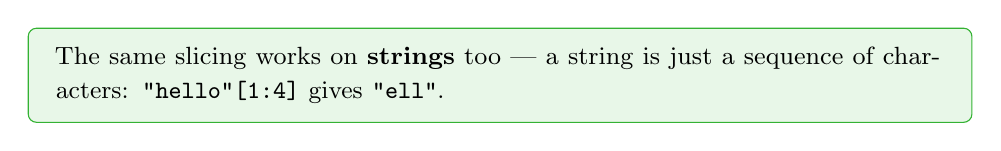
\begin{tikzpicture}
  \node[fill=lightgreen, draw=wurgreen, rounded corners=3pt, inner xsep=10pt, inner ysep=7pt, text width=\textwidth-24pt]{%
    {\small The same slicing works on \textbf{strings} too --- a string is just a sequence of
    characters: \texttt{"hello"[1:4]} gives \texttt{"ell"}.}};
\end{tikzpicture}
\end{frame}

\begin{frame}{Dictionaries}
\vspace{0.2cm}
{\small A \textbf{dictionary} stores \textbf{key $\rightarrow$ value} pairs. Instead of position,
you look things up by a \emph{key}. Perfect for word counts, settings, records.}
\medskip
\codebox{%
counts \textcolor{codegray}{=} \{\textcolor{codegreen}{"cat"}: \textcolor{codeorange}{3}, \textcolor{codegreen}{"dog"}: \textcolor{codeorange}{5}\}\\[6pt]
counts[\textcolor{codegreen}{"cat"}]\quad\ \ \ \ \ \textcolor{codegray}{\# 3  (look up by key)}\\
counts[\textcolor{codegreen}{"bird"}] \textcolor{codegray}{=} \textcolor{codeorange}{2}\quad\textcolor{codegray}{\# add a new pair}\\
counts[\textcolor{codegreen}{"cat"}] \textcolor{codegray}{=} \textcolor{codeorange}{4}\quad\ \textcolor{codegray}{\# update a value}\\[6pt]
counts.\textcolor{codeblue}{keys}()\quad\ \textcolor{codegray}{\# all keys}\\
counts.\textcolor{codeblue}{values}()\quad\textcolor{codegray}{\# all values}}
\medskip
{\small\textcolor{midgray}{\textit{Keys are usually strings; values can be anything. Dictionaries
are everywhere in data work.}}}
\end{frame}

\begin{frame}{Tuples \& Sets (Briefly)}
\vspace{0.3cm}
\begin{columns}[T]
  \column{0.48\textwidth}\vspace{0pt}
  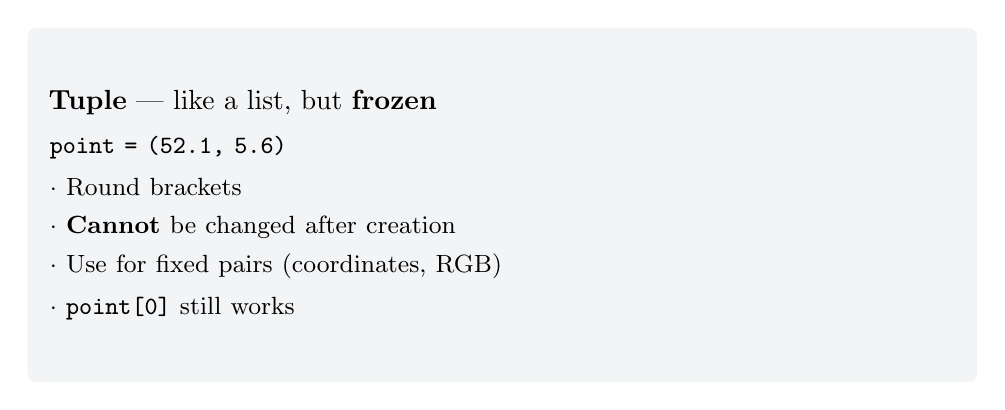
\begin{tikzpicture}
    \node[fill=lightgray, rounded corners=3pt, inner xsep=8pt, inner ysep=8pt, text width=\columnwidth-18pt, minimum height=4.5cm]{%
      \textbf{Tuple} --- like a list, but \textbf{frozen}\\[5pt]
      {\small
      \texttt{point = (52.1, 5.6)}\\[4pt]
      $\cdot$ Round brackets\\[3pt]
      $\cdot$ \textbf{Cannot} be changed after creation\\[3pt]
      $\cdot$ Use for fixed pairs (coordinates, RGB)\\[3pt]
      $\cdot$ \texttt{point[0]} still works}};
  \end{tikzpicture}
  \column{0.48\textwidth}\vspace{0pt}
  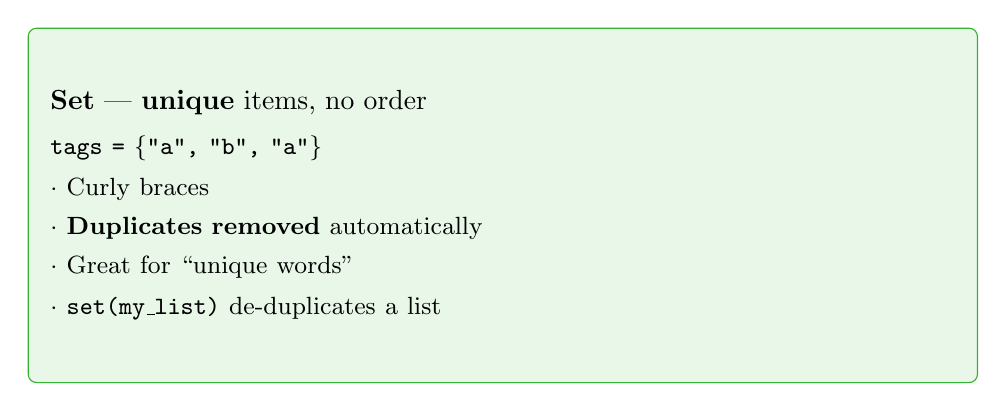
\begin{tikzpicture}
    \node[fill=lightgreen, draw=wurgreen, rounded corners=3pt, inner xsep=8pt, inner ysep=8pt, text width=\columnwidth-18pt, minimum height=4.5cm]{%
      \textbf{Set} --- \textbf{unique} items, no order\\[5pt]
      {\small
      \texttt{tags = \{"a", "b", "a"\}}\\[4pt]
      $\cdot$ Curly braces\\[3pt]
      $\cdot$ \textbf{Duplicates removed} automatically\\[3pt]
      $\cdot$ Great for ``unique words''\\[3pt]
      $\cdot$ \texttt{set(my\_list)} de-duplicates a list}};
  \end{tikzpicture}
\end{columns}
\medskip
{\small\textcolor{midgray}{\textit{Remember the ``types vs.\ tokens'' idea? \texttt{set(words)}
turns a list of tokens into the set of unique types.}}}
\end{frame}

\begin{frame}{Module 2: Takeaways}
\vspace{0.3cm}
\begin{itemize}\setlength\itemsep{8pt}
  \item[\textcolor{wurgreen}{\faCheck}] \textbf{Lists} \texttt{[...]}: ordered, changeable; index with \texttt{[0]}, slice with \texttt{[1:3]}
  \item[\textcolor{wurgreen}{\faCheck}] \textbf{Indexing starts at 0}; \texttt{-1} is the last item
  \item[\textcolor{wurgreen}{\faCheck}] \textbf{Dictionaries} \texttt{\{key: value\}}: look up by key, not position
  \item[\textcolor{wurgreen}{\faCheck}] \textbf{Tuples} \texttt{(...)}: like lists but unchangeable
  \item[\textcolor{wurgreen}{\faCheck}] \textbf{Sets} \texttt{\{...\}}: unordered collections of unique items
\end{itemize}
\medskip
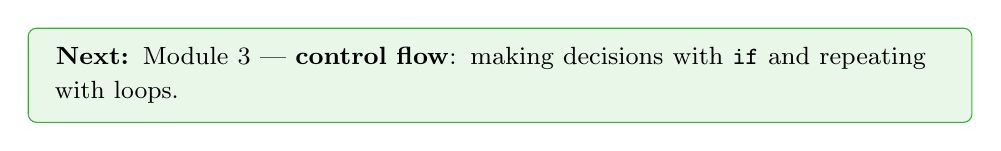
\begin{tikzpicture}
  \node[fill=lightgreen, draw=wurgreen, rounded corners=3pt, inner xsep=10pt, inner ysep=7pt, text width=\textwidth-24pt]{%
    {\small \textbf{Next:} Module 3 --- \textbf{control flow}: making decisions with \texttt{if}
    and repeating with loops.}};
\end{tikzpicture}
\end{frame}
\end{document}
